% Created 2017-09-11 Mon 14:46
\documentclass[9pt,lineo]{elife}

\usepackage{amsmath}
\usepackage{amssymb}
\usepackage[version=4]{mhchem}
\usepackage{siunitx}


              \usepackage[utf8]{inputenc}
\sisetup{detect-all}
\setcounter{secnumdepth}{0}
\date{\today}
\title{}
\hypersetup{
 pdfauthor={},
 pdftitle={},
 pdfkeywords={},
 pdfsubject={},
 pdfcreator={Emacs 25.1.2 (Org mode 8.3.5)}, 
 pdflang={English}}
\begin{document}

\begin{figure}
  \begin{fullwidth}
\centering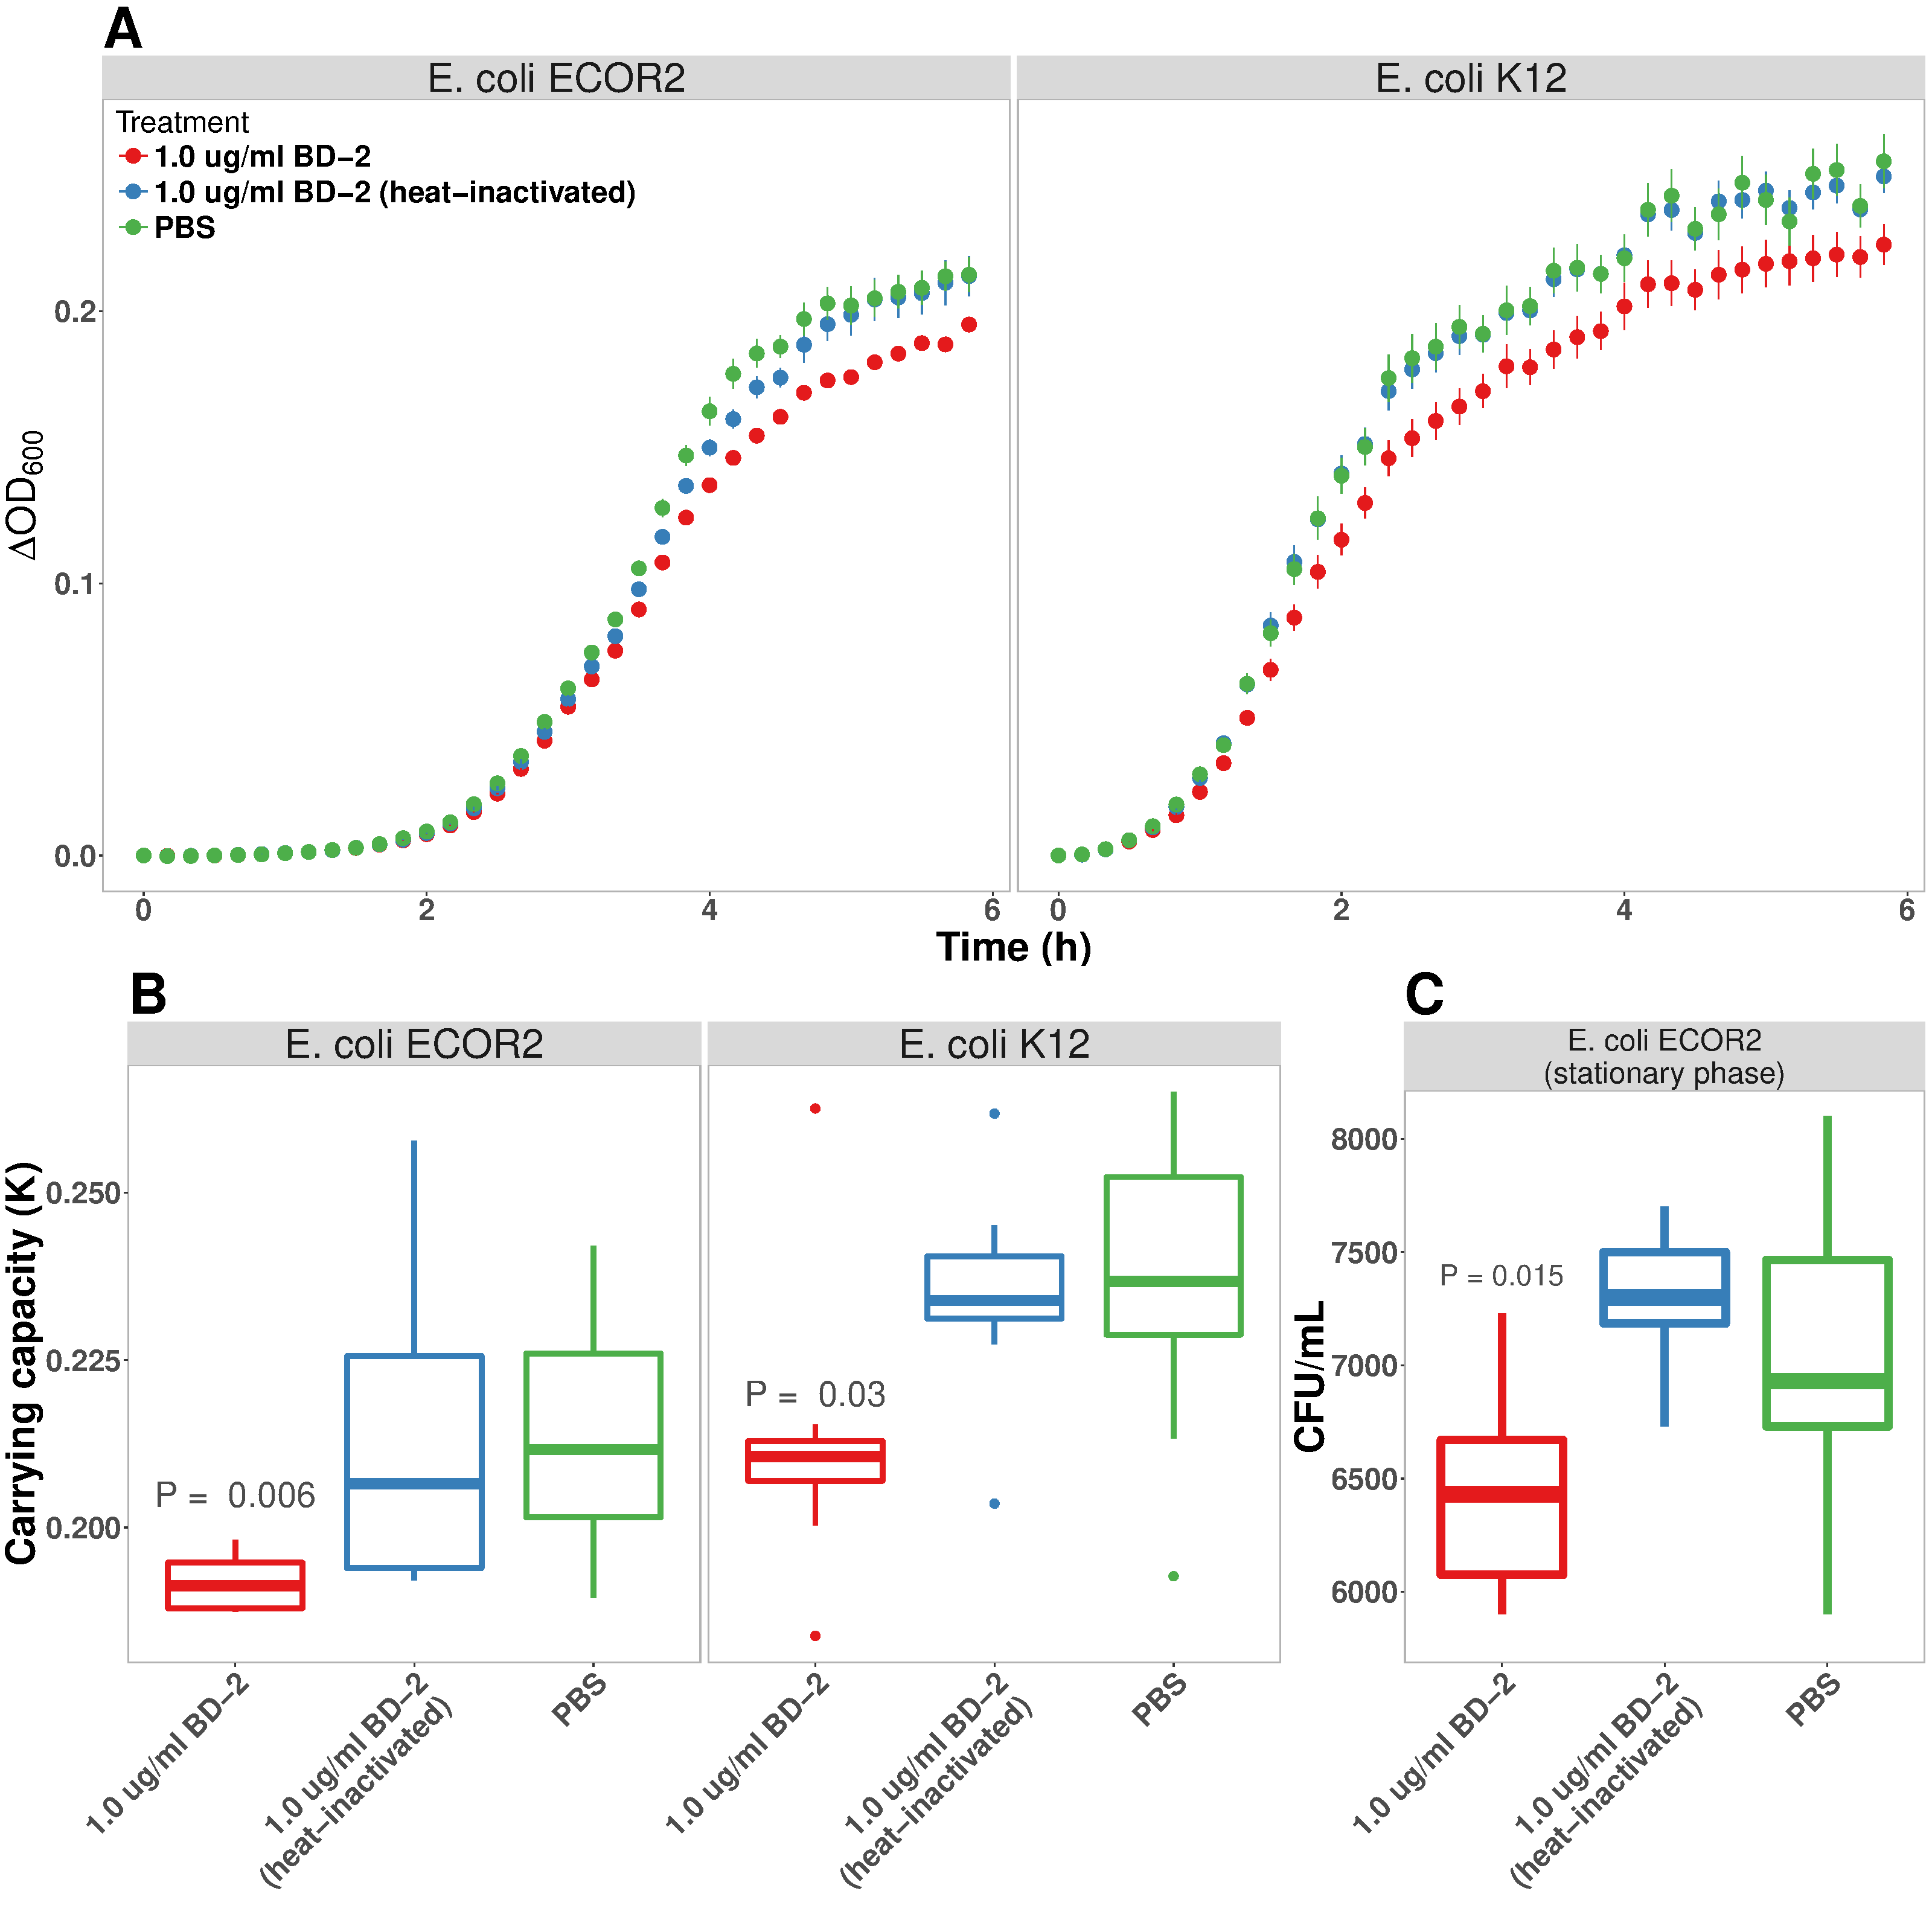
\includegraphics[width=0.9\linewidth]{./figures/figure6/figure6_supplement2.pdf}    
 \caption*{\textbf{Figure 6 - Supplement 2. } \textbf{A} Optical density (600 nm) of \textit{E. coli} str. ECOR2 and \textit{E. coli} str. K12 suspension cultures supplemented with PBS, BD-2 (1 $\mu$g/ml), or heat-inactivated BD-2 at 10 min intervals over a 6 h period at \SI{37}{\celsius}. \textbf{B} Carrying capacity (\textit{K}) of \textit{E. coli} cultures incubated  with  PBS, BD-2 (1 $\mu$g/ml), or heat-inactivated BD-2 during log-phase growth (panel A). \textit{P} values represents the results of a one-tailed Student's \textit{t}-test relative to PBS treatment. For panels A and B, \textit{N} = 8 per experimental condition for each \textit{E. coli} strain. \textit{C} CFU/ml of late stationary phase \textit{E. coli} str. ECOR2 cultures diluted in PBS and supplemented with BD-2 (1 $\mu$g/ml) or heat-inactivated BD-2 for 6 h at \SI{37}{\celsius}. \textit{N} = 8 (BD-2 and heat inactivated BD-2) or 16 (PBS).}
\label{fig:fullwidth}
\end{fullwidth}
\end{figure}
\end{document}